\section{Preliminary experiments}
\label{sec:experiments}

Our experimental analysis addresses four questions:
(1) How does CORELS' accuracy compare to other algorithms?
(2) How rapidly does the objective function converge?
(3) How rapidly does CORELS prune the search space?
(4) How much does each of the implementation optimizations contribute to CORELS' performance?
All results presented use the COMPAS data set unless otherwise noted,
and were executed on (describe machine) \dots

We first ran a 10-fold cross validation experiment using CORELS and eight other algorithms:
GLM, SVM, AdaBoost, CART, C4.5, RF, RIPPER, and scalable rule lists (SBRL).
There were no statistically significant differences in the accuracies of the different
algorithms. In fact, the difference between folds was far larger than the difference
between algorithms. We conclude that CORELS produces models whose accuracy is comparable
to those found via other algorithms.

Figure \ref{fig:objective} illustrates how both the objective and the size of
the remaining search space decrease as CORELS executes.
The objective drops quickly, achieving the optimal value within 10 seconds.
CORELS certifies optimality in less than 6 minutes --
the objective lower bound of the remaining search space
monotonically converges to the optimal objective
as the search space steadily shrinks.

Finally, we determine the efficacy of each of our data structure and bounding
optimizations.
Table \ref{tab:ablation} provides sumary statistics for experiments using
the full CORELS implementation and implementations with a specific
optimization removed.
Figure \ref{fig:queue} presents a view of the same experiments, focusing
on just three of the optimizations. These charts depict the number of rule
lists of a given length in the queue during the algorithm's execution.

\begin{figure}[t!]
\begin{center}
%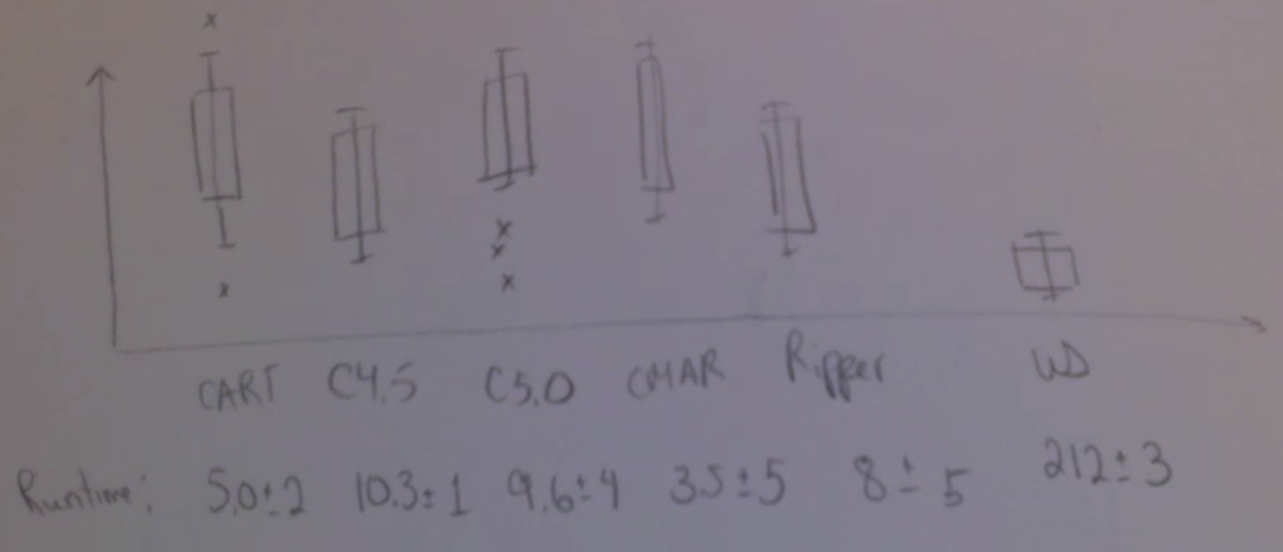
\includegraphics[width=0.75\textwidth]{figs/sketch-comparison.png}
\begin{arxiv}
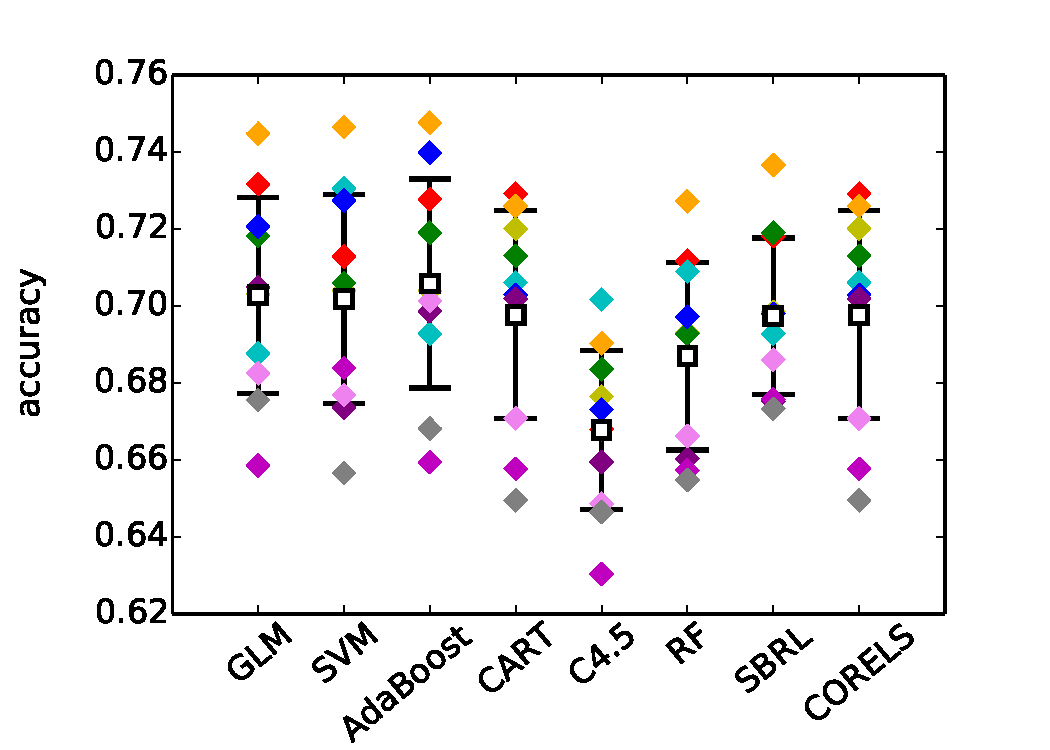
\includegraphics[width=0.75\textwidth]{figs/compare-compas.pdf}
\end{arxiv}
\begin{kdd}
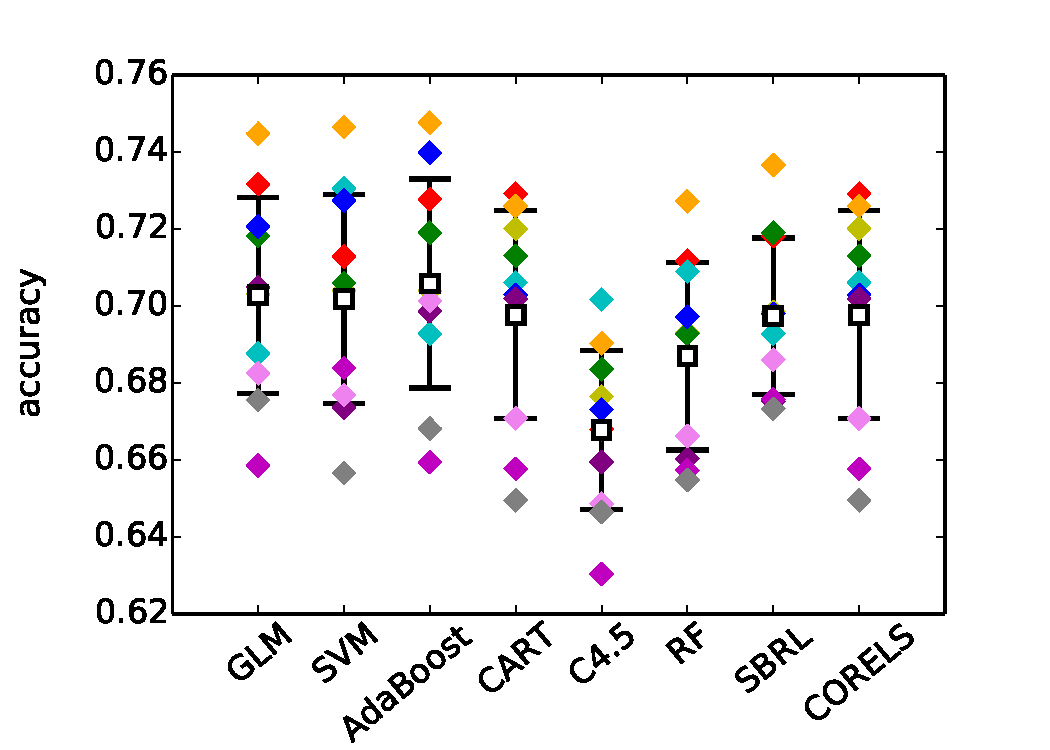
\includegraphics[width=0.4\textwidth]{figs/compare-compas.pdf}
\end{kdd}
\end{center}
\caption{Comparison with other methods:
Test error for us and a few other algorithms
(CART, C4.5, CBA, CMAR/CPAR, C5.0, Ripper, \dots),
as a function of sparsity over 10 folds, for one big dataset (box plots).
Also report algorithm runtimes (mean $\pm$ standard deviation over 10 folds).}
\label{fig:comparison}
\end{figure}

\begin{arxiv}
\begin{figure}[t!]
\begin{center}
\end{center}
\caption{Missing:  Test error as a function of regularization and sparsity
(number of rules) as a function of regularization, over 10 folds,
for one big dataset.}
\label{fig:regularization}
\end{figure}
\end{arxiv}

\begin{arxiv}
\begin{figure}[t!]
\begin{center}
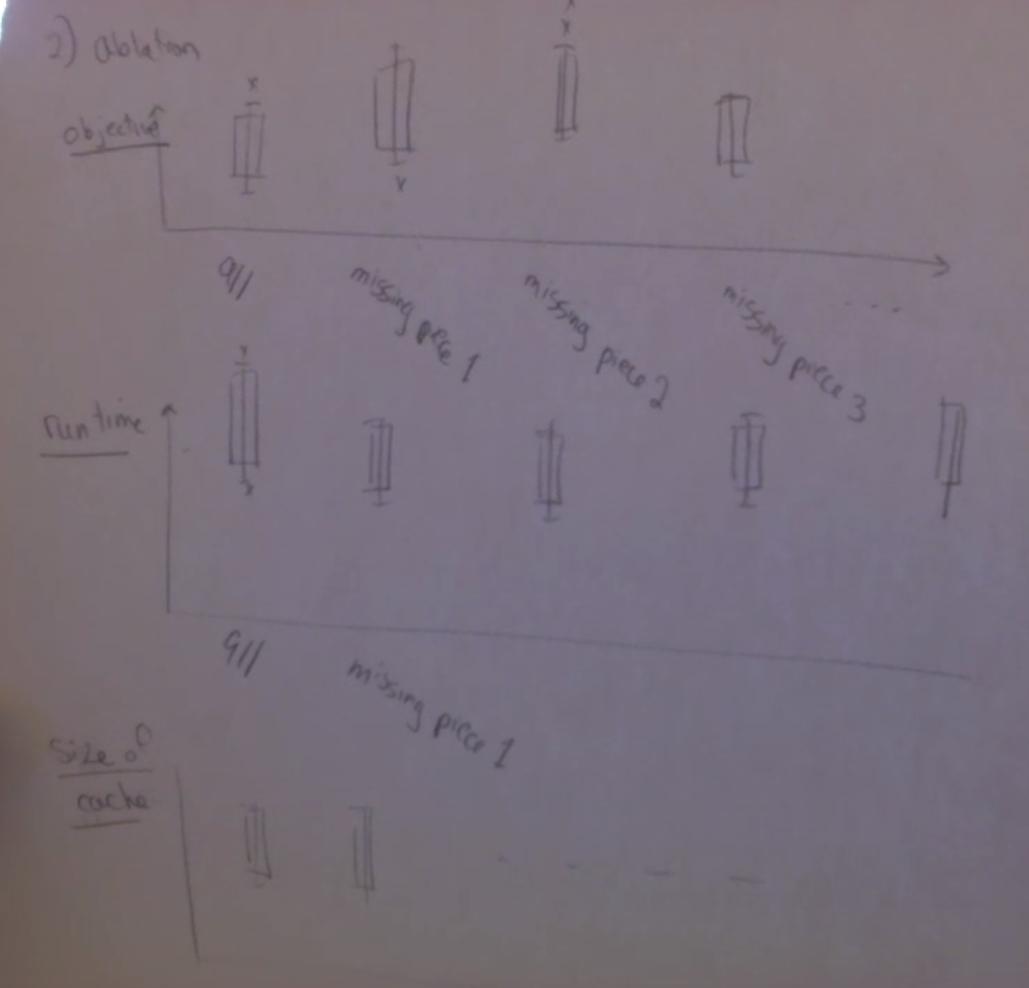
\includegraphics[width=0.75\textwidth]{figs/sketch-ablation.png}
\end{center}
\caption{Ablation experiment:
Show the effect of each ``piece'' at a time,
run X without each in turn and show the difference in either
quality of solution or runtime or amount of memory, size of cache or queue,
where X is a specific implementation
(meaning a specific scheduling policy and node type)}
\label{fig:ablation}
\end{figure}
\end{arxiv}

\begin{arxiv}
\begin{figure}[t!]
\begin{center}
\end{center}
\caption{Missing:  Some sort of comparison of different scheduling policies}
\label{fig:scheduling-policy}
\end{figure}
\end{arxiv}

\begin{arxiv}
\begin{figure}[t!]
\begin{center}
%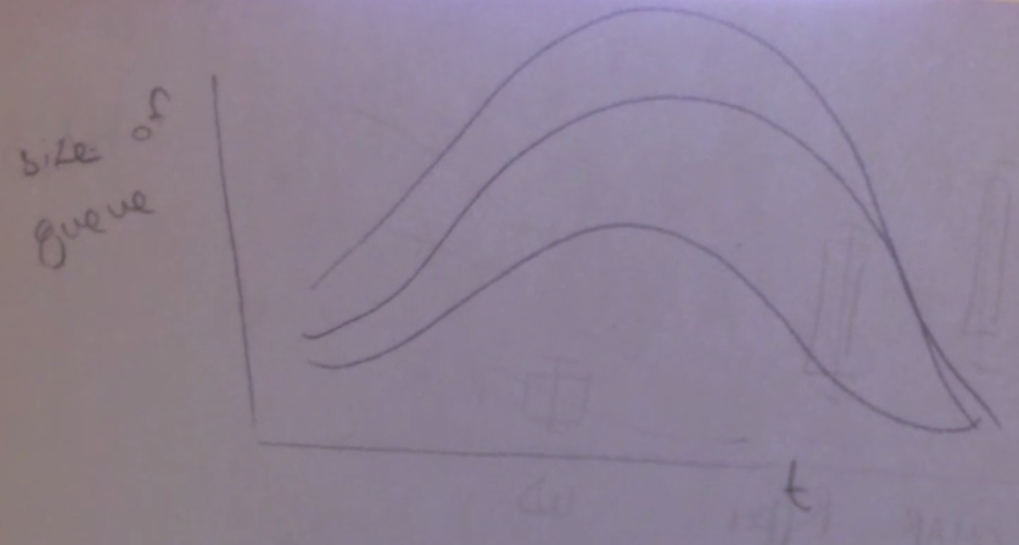
\includegraphics[width=0.65\textwidth]{figs/sketch-queue-size.png}
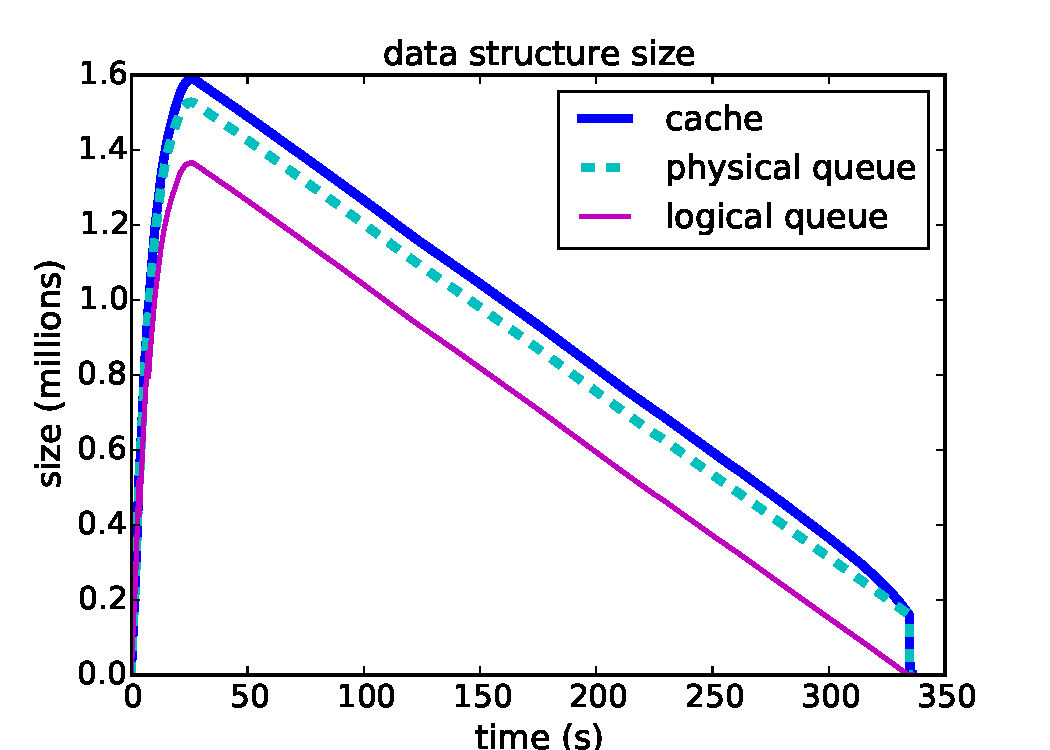
\includegraphics[width=0.8\textwidth]{figs/ela_compas-queue-cache-size-insertions.pdf}
\end{center}
\caption{Cache and queue data structure sizes and insertions.
%
The top plot shows the sizes of the cache and queue data structures,
as a function of wall clock time.
%
The number of nodes in the cache (solid black line) is an
upper bound on the number of elements in the physical queue
(dotted gray line), since the physical queue elements only
correspond to the cache trie data structure's leaf nodes
plus disconnected cache nodes that have been marked for deletion.
%
The queue's physical size is an upper bound on its
logical size (solid blue line), which doesn't include nodes
that have been marked for deletion.
%
The bottom plot shows the cumulative number of cache insertions,
which is equivalent to the cumulative number of queue insertions,
as a function of wall clock time.
}
\label{fig:queue-cache-size-insertions}
\end{figure}
\end{arxiv}

\begin{figure}[t!]
\begin{center}
%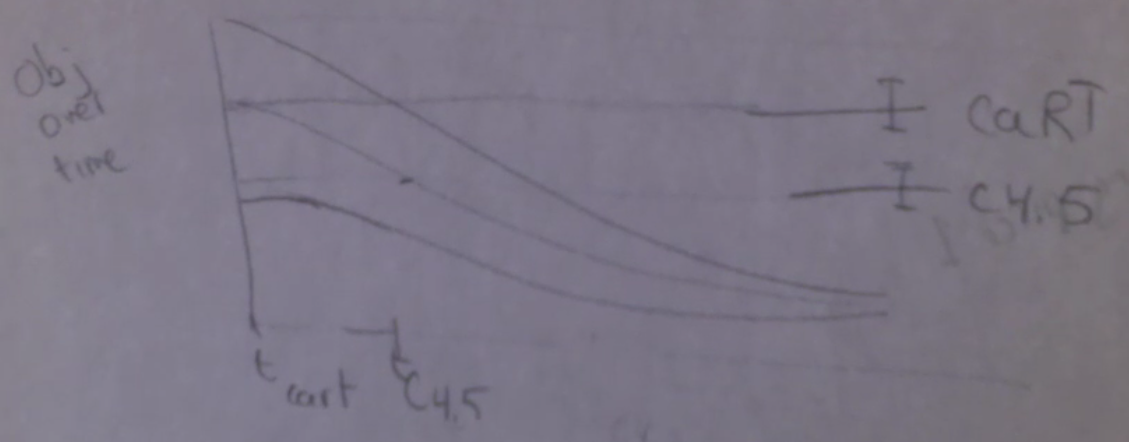
\includegraphics[width=0.65\textwidth]{figs/sketch-objective.png}
\begin{arxiv}
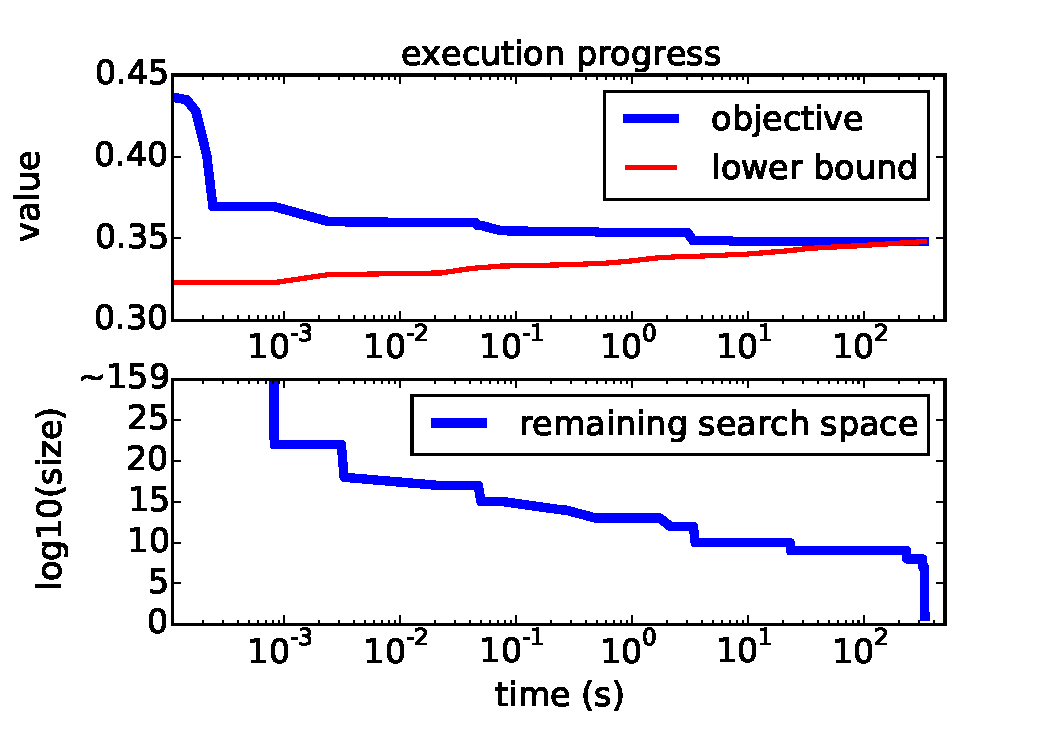
\includegraphics[width=0.8\textwidth]{figs/ela_compas-remaining-space.pdf}
\end{arxiv}
\begin{kdd}
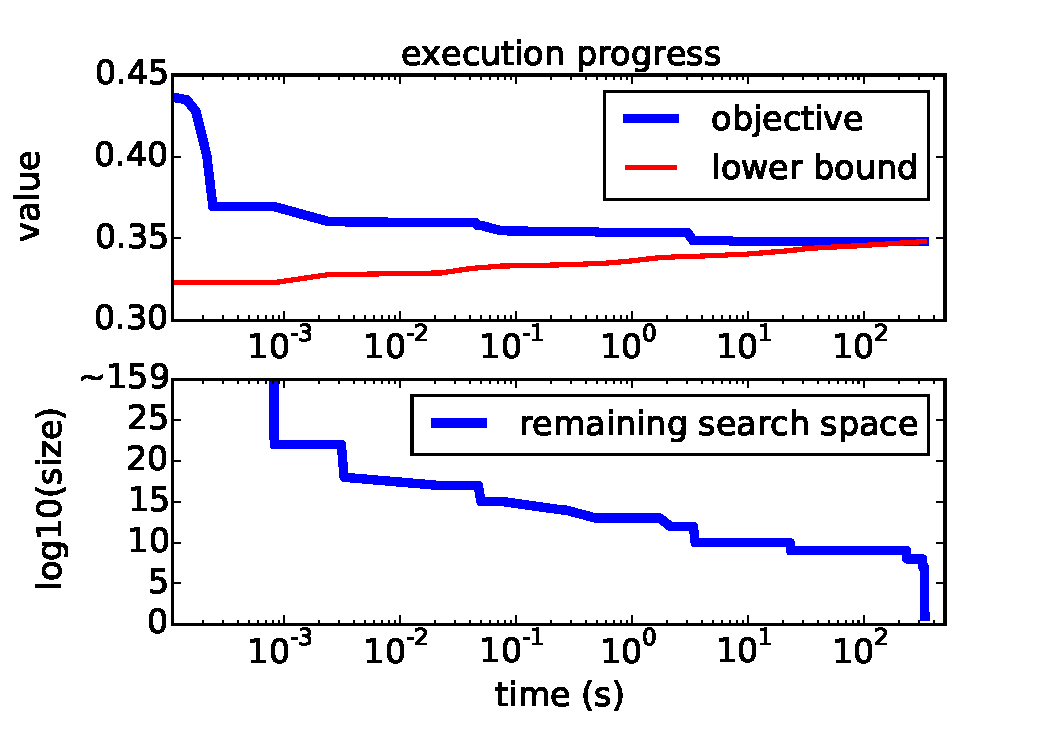
\includegraphics[width=0.4\textwidth]{figs/ela_compas-remaining-space.pdf}
\end{kdd}
\end{center}
\caption{Top: Objective value and lower bound as a function of wall clock time.
%
Missing: horizontal lines and x-ticks for CART and C4.5.
%
Bottom:
The logarithm (base 10) of the upper bound
from Proposition~\ref{prop:remaining-eval-coarse}
on the size of the remaining search space,
as a function of wall clock time.
%
This bound depends on the total number of available rules,
as well as two dynamic quantities:
the current best objective value,
and the histogram of logical queue elements,
partitioned by prefix length.}
\label{fig:objective}
\end{figure}

\begin{table}[t]
\centering
\begin{tabular}{l | c | c | c | c | c}
Ablated & $t_\text{total}$ & $t_\text{opt}$ & $K_\text{max}$ & $i_\text{total}$ & $\max | Q |$ \\
component & (s) & (s) & & ($\times 10^6$) & ($\times 10^6$) \\
\hline
none & 336 & 7 & 6 & 1.61 & 1.37 \\
priority queue & 453 & 4 & 6 & 1.93 & 1.58 \\
support bounds & 580 & 11 & 6 & 2.38 & 2.06 \\
permutation map & 3634 & 19 & 6 & 15.0 & 14.1 \\
lookahead bound & 4401 & 8 & 7 & 19.5 & 17.7 \\
identical pts. bound & --- & 48 & $\ge 10$ & $>286$ & $>282$ \\
\end{tabular}
\vspace{2mm}
\caption{Ablation experiment.
Total time, time to optimum, maximum evaluated prefix length,
number of queue insertions, maximum queue size.}
\label{tab:ablation}
\end{table}

\begin{figure}[t!]
\begin{center}
\begin{arxiv}
%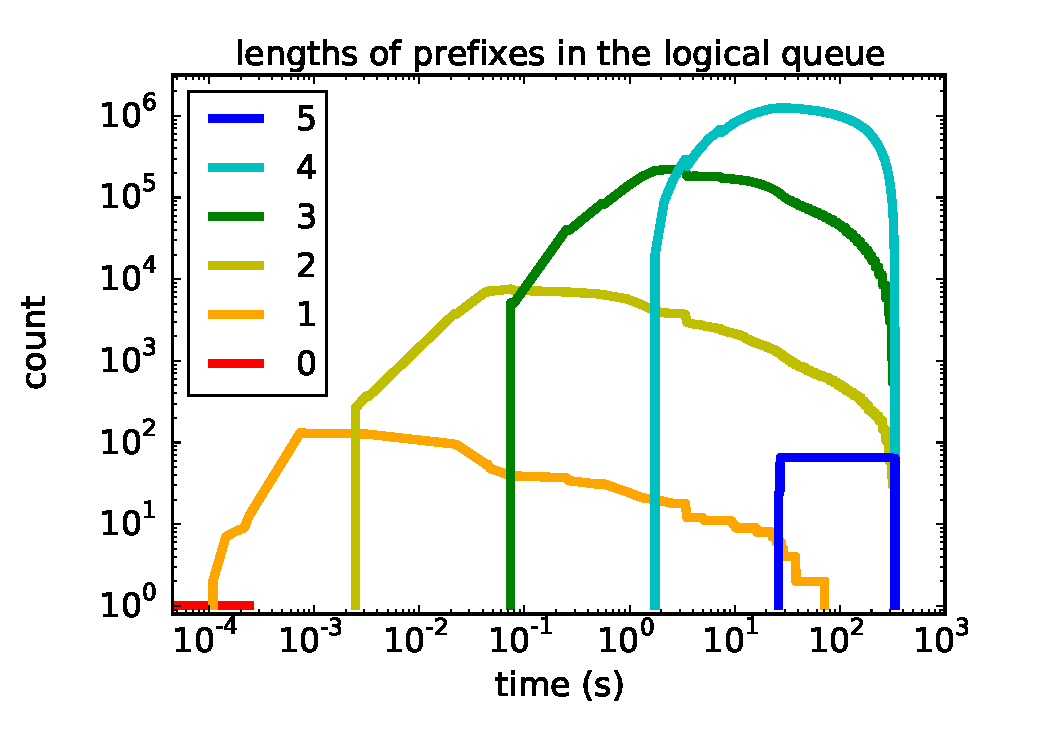
\includegraphics[width=0.8\textwidth]{figs/ela_compas-queue.pdf}
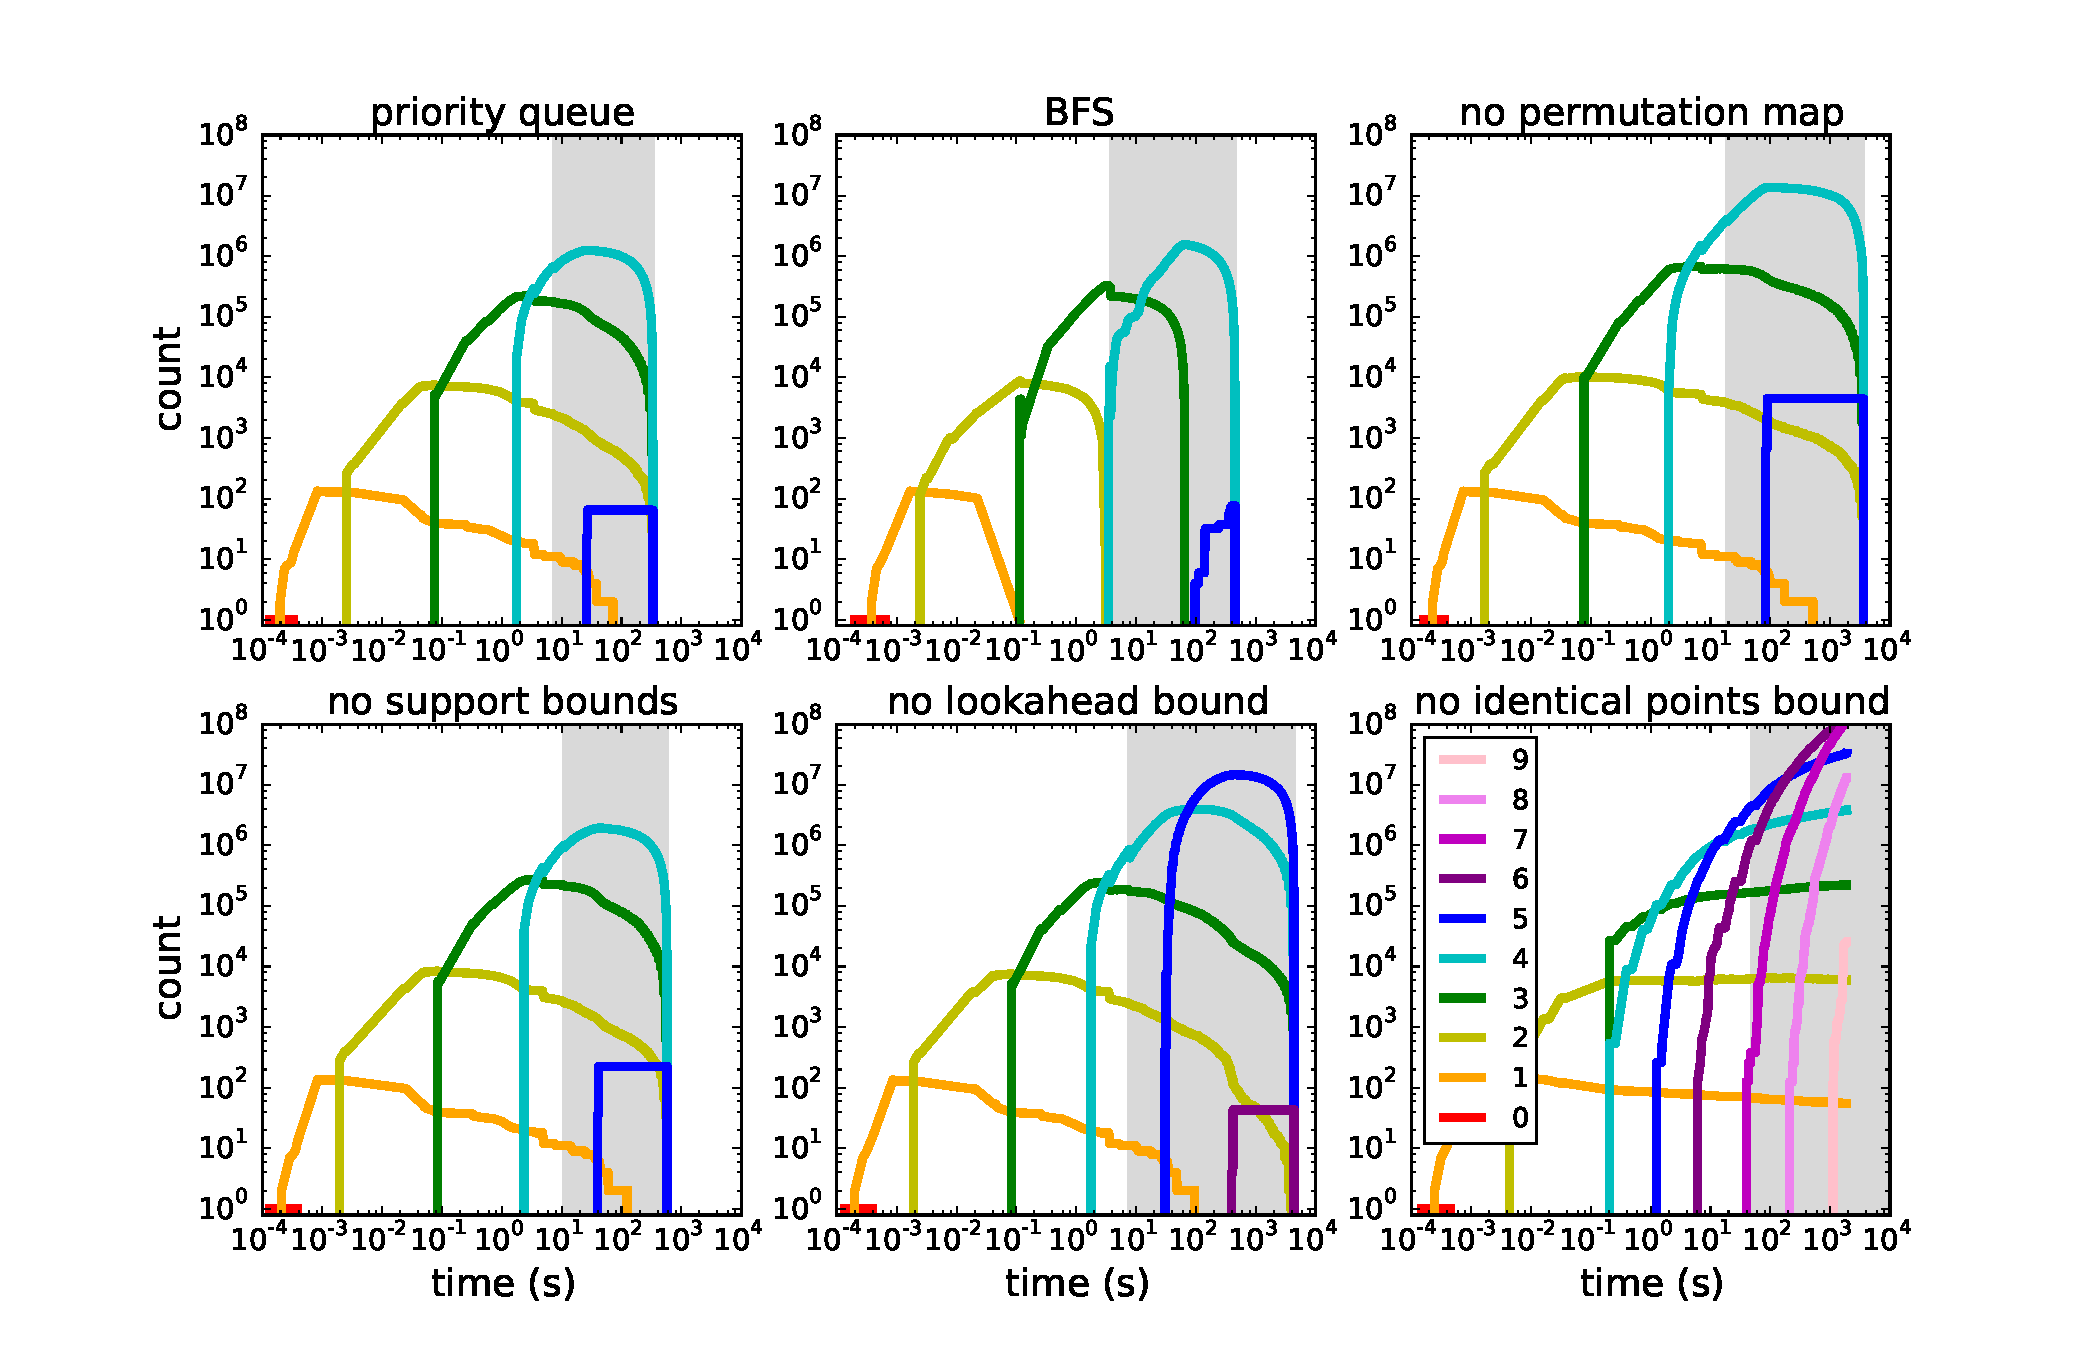
\includegraphics[width=\textwidth]{figs/ela_compas_compare-queue.pdf}
\end{arxiv}
\begin{kdd}
%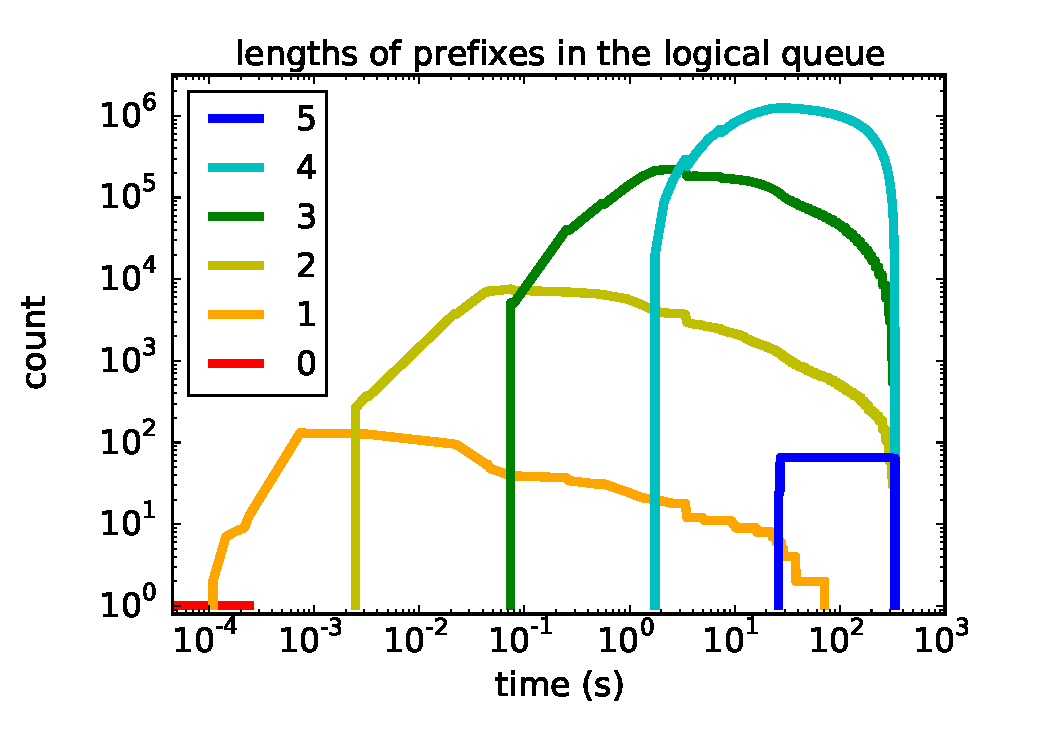
\includegraphics[width=0.5\textwidth]{figs/ela_compas-queue.pdf}
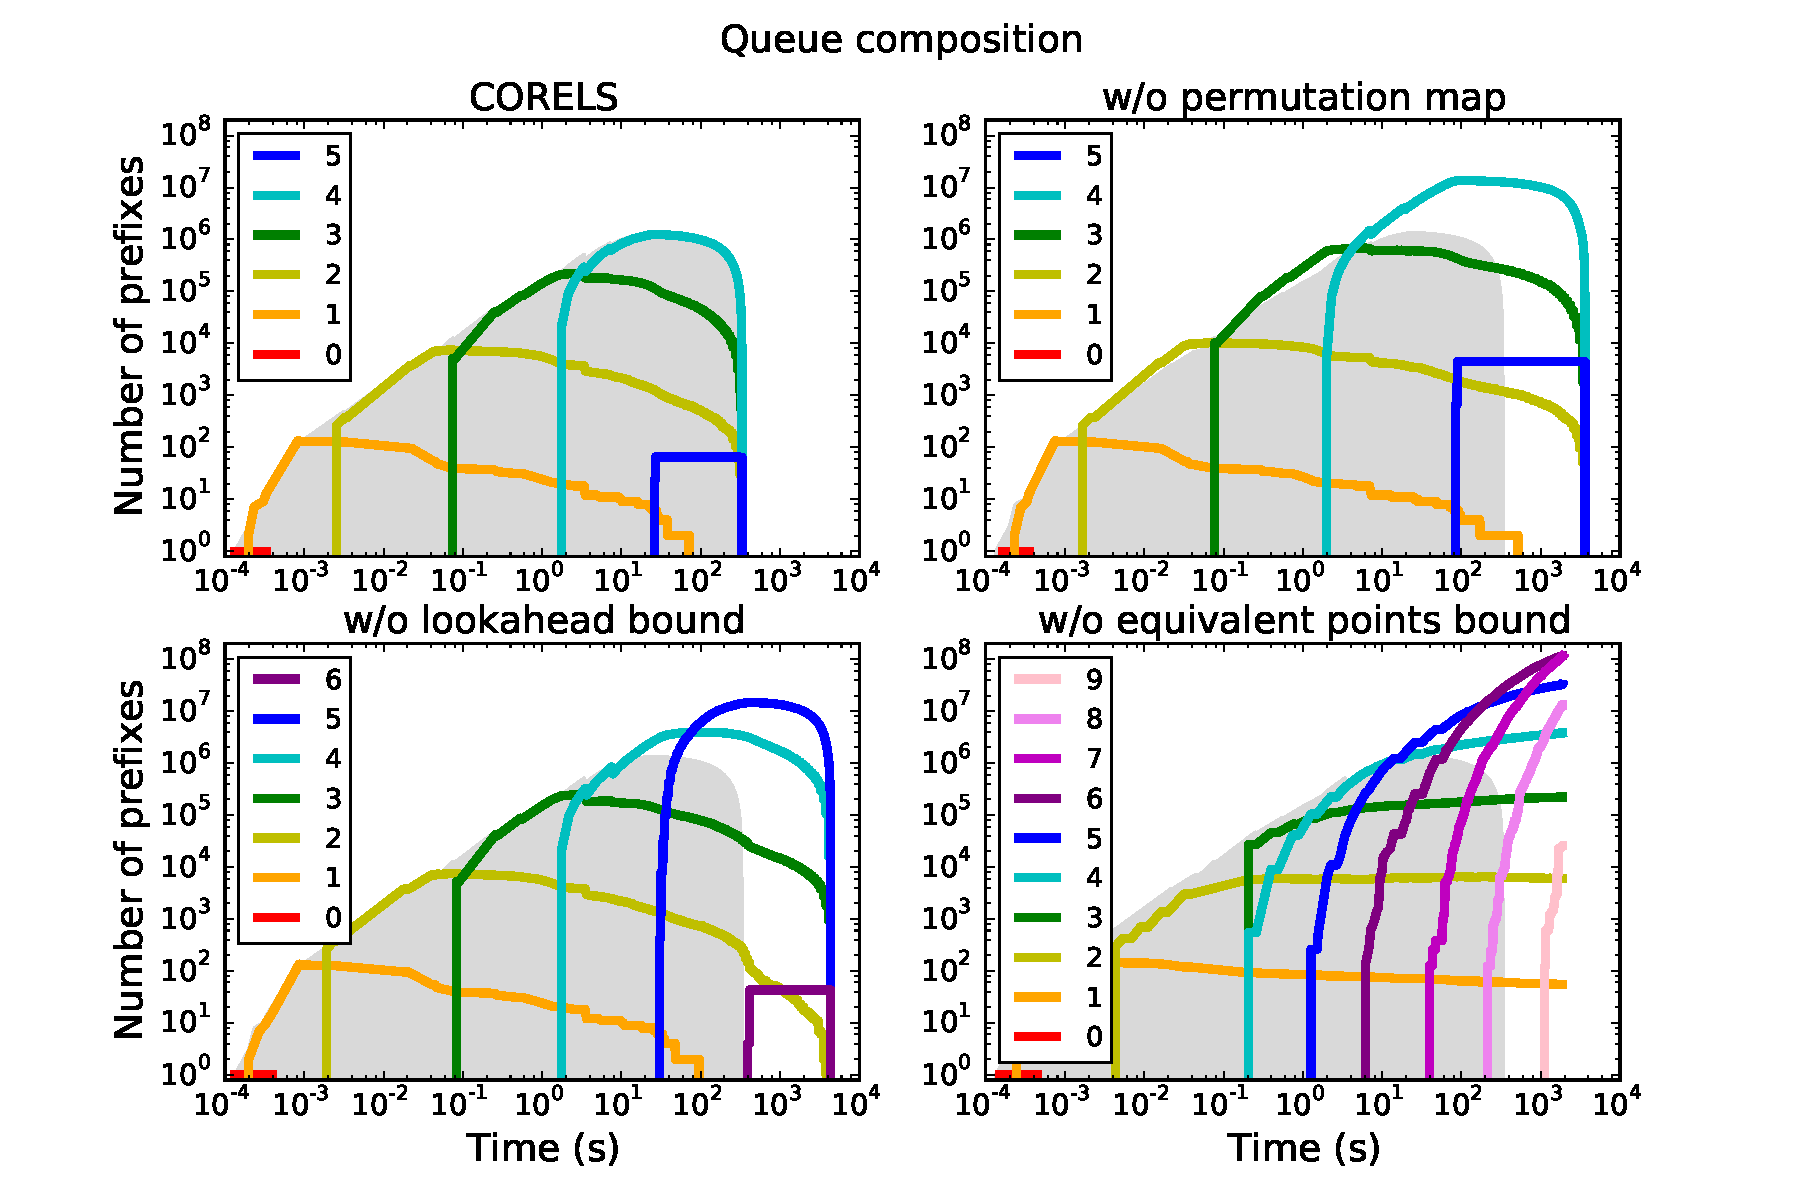
\includegraphics[trim={30mm 10mm 20mm 10mm}, width=0.5\textwidth]{figs/ela_compas_compare_small-queue.pdf}
\end{kdd}
\end{center}
\caption{Ablation experiment and logical queue composition.
Note the last experiment is incomplete and was run on a (different)
machine with a large amount of memory.  Was using about 136GB RAM when terminated.
}
\label{fig:queue}
\end{figure}

%\begin{figure}[t!]
%\begin{center}
%%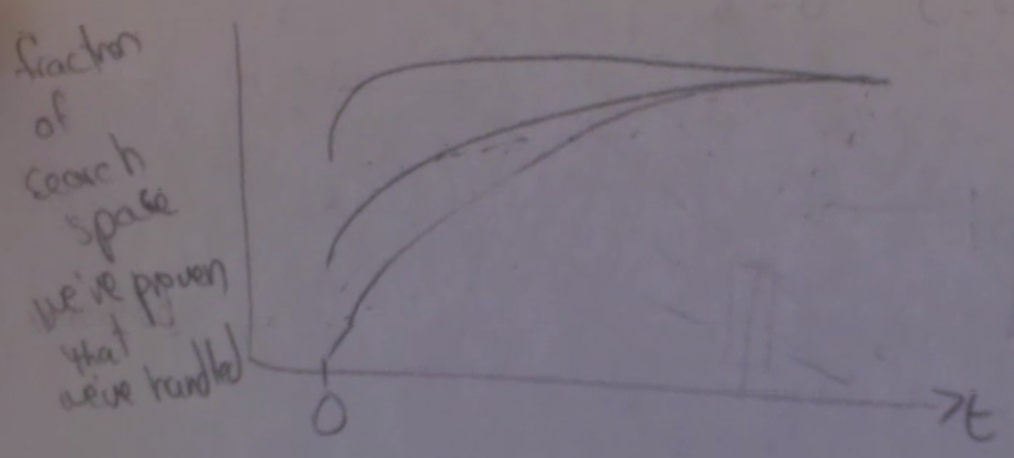
\includegraphics[width=0.65\textwidth]{figs/sketch-search-space.png}
%\begin{arxiv}
%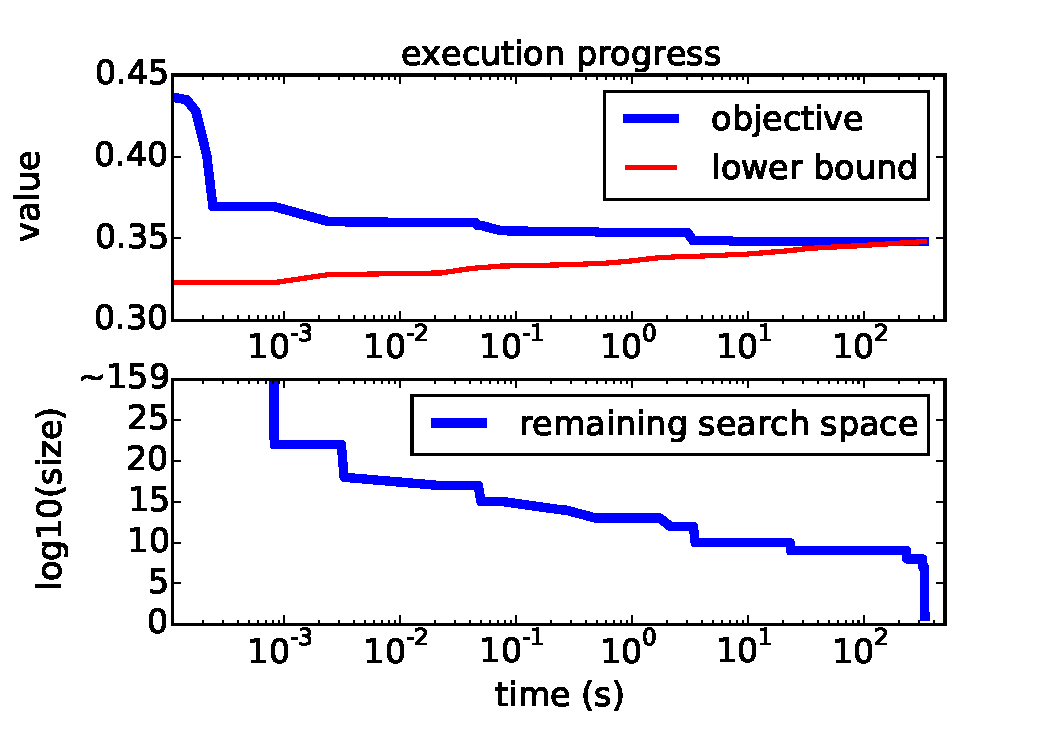
\includegraphics[width=0.8\textwidth]{figs/ela_compas-remaining-space.pdf}
%\end{arxiv}
%\begin{kdd}
%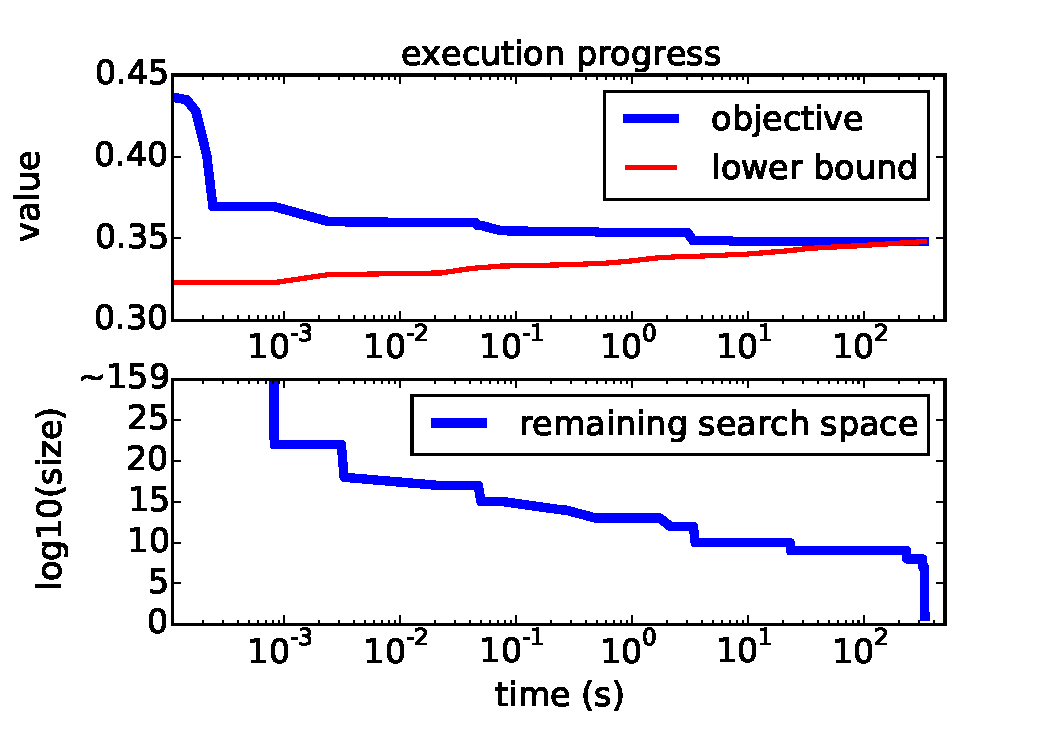
\includegraphics[width=0.5\textwidth]{figs/ela_compas-remaining-space.pdf}
%\end{kdd}
%\end{center}
%\caption{The logarithm (base 10) of the upper bound
%from Proposition~\ref{prop:remaining-eval-coarse}
%on the size of the remaining search space,
%as a function of wall clock time.
%%
%This bound depends on the total number of available rules,
%as well as two dynamic quantities:
%the current best objective value,
%and the histogram of logical queue elements,
%partitioned by prefix length.
%}
%\label{fig:search-space}
%\end{figure}

\begin{arxiv}
\begin{figure}[t!]
\begin{center}
%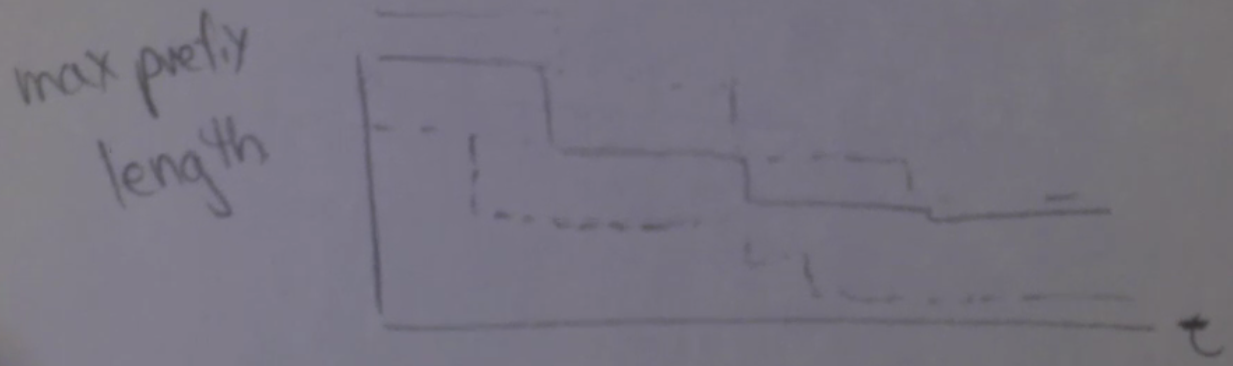
\includegraphics[width=0.65\textwidth]{figs/sketch-max-length.png}
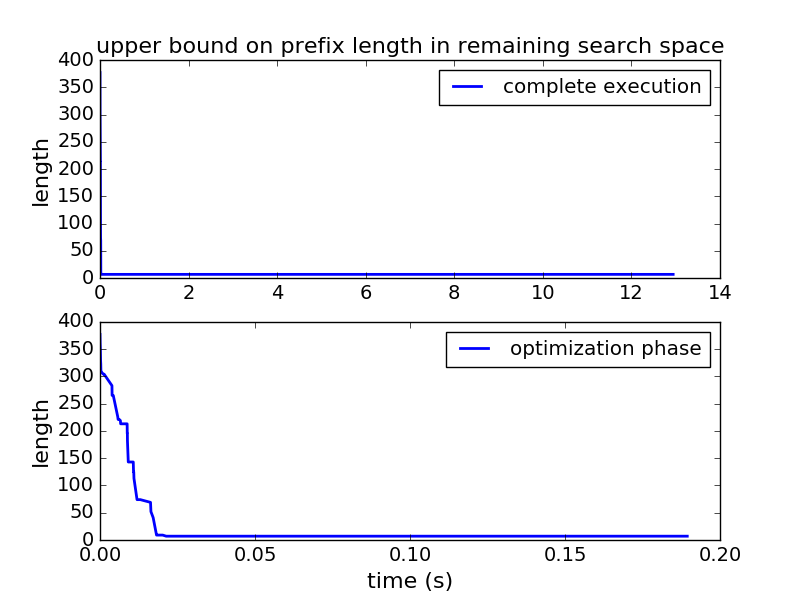
\includegraphics[width=0.8\textwidth]{figs/ela-max-length-check.png}
\end{center}
\caption{Max prefix length over time (computed from objective value)}
\label{fig:max-length}
\end{figure}

\begin{figure}[t!]
\begin{center}
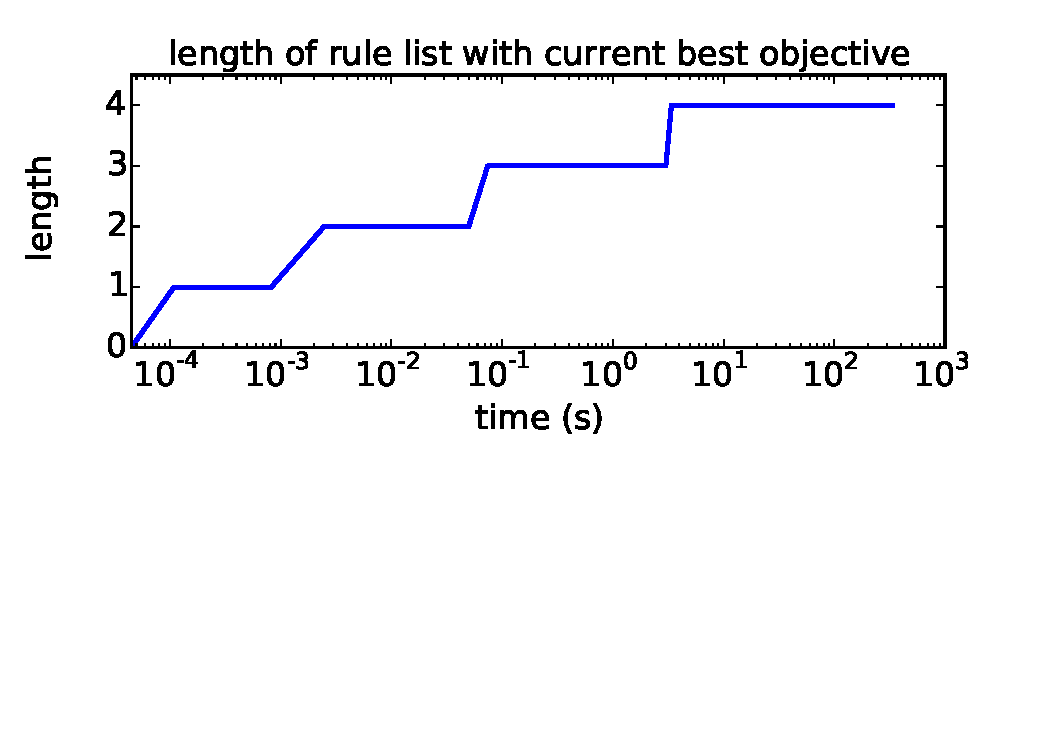
\includegraphics[width=0.8\textwidth]{figs/ela_compas-prefix-length.pdf}
\end{center}
\caption{Best prefix length over time}
\label{fig:prefix-length}
\end{figure}
\end{arxiv}
